% !TeX spellcheck = en_GB
\section{Question 3}

\subsection{A)}
\begin{quote}
	\textit{"Assume	that	the	data	from	project	3	is	not	a	massive	data	set,	but	a	data	stream.	Every	time	step,	a	large	collection	of	vehicles	and	persons	is	generated	(based	on	the	attributes	contained	in	the	<vehicle>	and	<person>	elements	of	the	XML	file	given	in	project	3).	How	would	you	proceed	to	characterize	such	a	data	stream?"}
\end{quote}
To characterize a stream of data I would look at at least three factors; structure, mean throughput and peek throughput. 

In project 3 the data of the stream contains structured data since it is in XML format. The structure is as follows:
\begin{verbatim}
<Timestep>
    <vehicle, id, x, y, angle, type, speed, pos, lane, slope/>
</Timestep>
\end{verbatim}
or 
\begin{verbatim}
<Timestep>
    <person, id, x, y, angle, speed, pos, edge/>
</Timestep>
\end{verbatim}
depending on which type the input has. In general when working with XML, the structur is easily obtained since the structure of the data is part of the data itself. Had the data been in JSON format it would be more difficult, albeit not impossible to find this structure, and had the data been unstructured it would have been even more difficult, since one should try to create and fit a schema at the same time.

The mean throughput can be described as the average of the number of discrete elements over a timeunit. Often when working with infinite streams we need to specify and limit that time to base this over. This could be calculated either with batch jobs, but it could also be calculated using windowed stream analysis. By examining a window in the stream one could approximate the average amount of entities pr timesteps. This approximation of the overall mean throughput would probably also be more describing than an overall mean, since streams are infinite and ever changing. The overall mean would not be representative for the stream currently, and it would therefore be a bad foundation to base decisions on.

\newpar The third characterization could be the peek amount of elements in the stream, which could be approximated by comparing the current mean throughput with the last mean throughput. By using the mean instead of hard values, the computation is less sensitive to very short peeks, which might or might not be desired. This value could have some kind of fallout value (for example a day or a week), such that it continues to be representative and a former peek does not continue to overshadow the current reality. The peek value can be used to help the developers decide on whether to scale the system, or rent extra computation in small periods of time, as it is for example seen possible with AWS\footnote{https://aws.amazon.com/} or Azure\footnote{https://azure.microsoft.com/en-us/?b=16.48}.

\subsection{B)}
\begin{quote}
		\textit{"Describe	a	meaningful	view	based	on	the	data	set	from	the	Project	2	data	set.	How	do	you	obtain	that	view?	Describe	the	problems	you	faced	obtaining	such	views	in	project	2	and	how	you	fixed	them."}
\end{quote}
I have chosen to showcase the second view from our Project 2 as I find that the most interesting. The view was described as follows: 
\begin{quote}
	\textit{"How can Wi-Fi data be used for tracking an individual at ITU?"}
\end{quote}
The hypothesis is that information about what access points a client has been connected to makes it possible to track a single person at ITU. Since each Wi-Fi client has an unique ID in the data set, tracking that ID around the ITU through various access points in certain rooms, one could connect this information to teaching activities. One could essentially build a schedule corresponding to a person, the holder of the unique ID, and by cross referencing the public course base, identify any student or teacher. 

It is necessary to assume that every person is connected to Wi-Fi whenever they are at ITU and even more important that they are connected to the access points in the rooms that they have courses in. 

\newpar To obtain the data we created a map-reduce program. The main part of the analysis is done in a mapper. The map method can be seen in figure \ref{code:project2_mapper}. The mapper joins the reading with its WiFi Client if it can, then it filters, the reading based on whether it measures the Access Point. Then for each reading, it joins it with the reading with its Access Point  and outputs the WifiClients id as the key and the location and time of that reading as the value. The mapper filters on null values for Access Points, and Locations.

\begin{figure}[H]
	
\begin{lstlisting}[frame=single, backgroundcolor=\color{light-gray}, basicstyle=\footnotesize\ttfamily, language=Java, numbers=left, numberstyle=\tiny \color{black}, breaklines=true]
public void map(AvroKey<Readings> key, NullWritable value, Context context) throws IOException, InterruptedException {
  Readings readings = key.datum();
  // Where
  if(wifiMap.containsKey(readings.getUUID().toString()))
  {
	// join
    WifiClient wifiClient = wifiMap.get(readings.getUUID().toString());
    // where
    if(wifiClient.getTypeOfMeasure().equals(WifiClientMeasure.AccessPoint))
    {
	  // select
      for(Reading reading : readings.getReadings())
      {
	    // join
        AccessPoint ap = apMap.get(reading.getValue());
        // where
        if(ap != null && ap.getLocationId() != null && locationMap.containsKey(ap.getLocationId()))
        {
          Date date = new Date(reading.getTimeStamp());
          Location location = locationMap.get(ap.getLocationId());
           
          context.write(new Text(readings.getUUID().toString()), new Text(location.getRoom() + "-" + dateFormat.format(date)));
        }
      }
    }
  }
}
\end{lstlisting}
\label{code:project2_mapper}
\caption{The map method for batch view 2 in project 2.}
\end{figure}

It becomes obvious that having this as one mapper does use the map-reduce framework to its full potential. It would have been a better idea to split this into multiple mappers, for example in the situation where the mapper iterates over the readings, it would have been smarter to use a mapper for that job. This could greatly increase the parallelism and therefore the scalability of the batch job.

The reducer simply aggregates the rooms, times together to a list over each specific WiFi client. A snippet of the output can be seen in figure \ref{fig:result_data}

\begin{figure}[H]
	\begin{lstlisting}[frame=single, backgroundcolor=\color{light-gray}, basicstyle=\footnotesize\ttfamily]
...
fd958189-5ad3-5586-a7ad-d3fe4e6f4695	
 4A32-2016-10-12:11, AUD44A60-2016-10-24:08, AUD44A60-2016-10-24:09, 
 AUD32-3A56-2016-10-04:09, AUD32-3A56-2016-10-04:08, 5A60-2016-10-12:07, 
 4A58-2016-10-24:08, AUD44A60-2016-10-10:09, AUD32-3A56-2016-10-04:10, 
 3A12-2016-10-06:11, 3A12-2016-10-06:12, 5A07-2016-10-12:11, 
 AUD32-3A56-2016-10-13:09, 5A05-2016-10-31:11, 5A07-2016-10-12:10,
 3A52-2016-10-25:11, 3A52-2016-10-25:10, AUD44A60-2016-10-24:10,
 4A58-2016-10-24:09, AUD44A60-2016-10-31:10, 4A16-2016-10-24:14,
 5A07-2016-10-05:08, 4A16-2016-10-24:11, 4A16-2016-10-24:13,
 4A16-2016-10-24:12, 5A07-2016-10-12:08, 5A07-2016-10-12:07,
 AUD32-3A56-2016-10-25:10, AUD44A60-2016-10-10:10, 4A58-2016-10-24:10,
 5A07-2016-10-12:09, 4A16-2016-10-10:12, 4A16-2016-10-10:11,
 4A16-2016-10-10:14, 4A16-2016-10-10:13, 4A22-2016-10-31:13,
 4A05-2016-10-12:11, AUD32-3A56-2016-10-06:09, AUD32-3A56-2016-10-13:10,
 5A07-2016-10-05:09, AUD32-3A56-2016-10-25:09,
...
	\end{lstlisting}
	\caption{Resulting data}
	\label{fig:result_data}
\end{figure}

\newpar Which can be represented a bit better visually in a schema as seen in figure \ref{fig:result_schema}.

\begin{figure}[H]
	\centering
	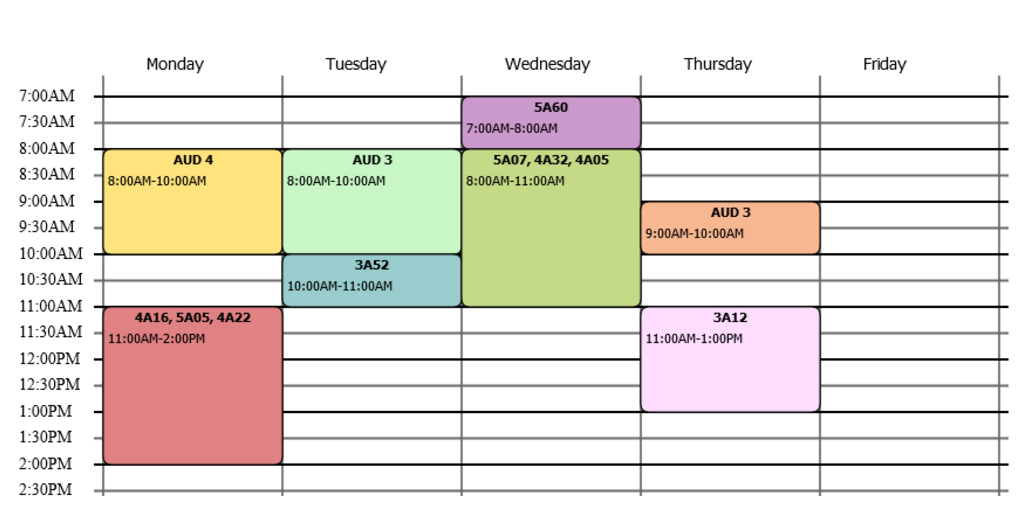
\includegraphics[width=\linewidth]{figures/schema-from-data.png}
	\caption{Resulting Schema}
	\label{fig:result_schema}
\end{figure}

\newpar With these results, the schema of a Wifi Client can be correlated to the schema of a student at ITU by matching it with course information and TimeEdit. If the Wifi Client has been to the rooms that match a student's schema then we might be able to specify which person, or at least which programme, a specific WiFi Client matches. For our result snippet shown above, the most plausible result is that the WiFi Client corresponds to a 1st year GBI student, since their schemas(see figure \ref{fig:timeedit_schema}) overlap nicely.

\begin{figure}[H]
	\centering
	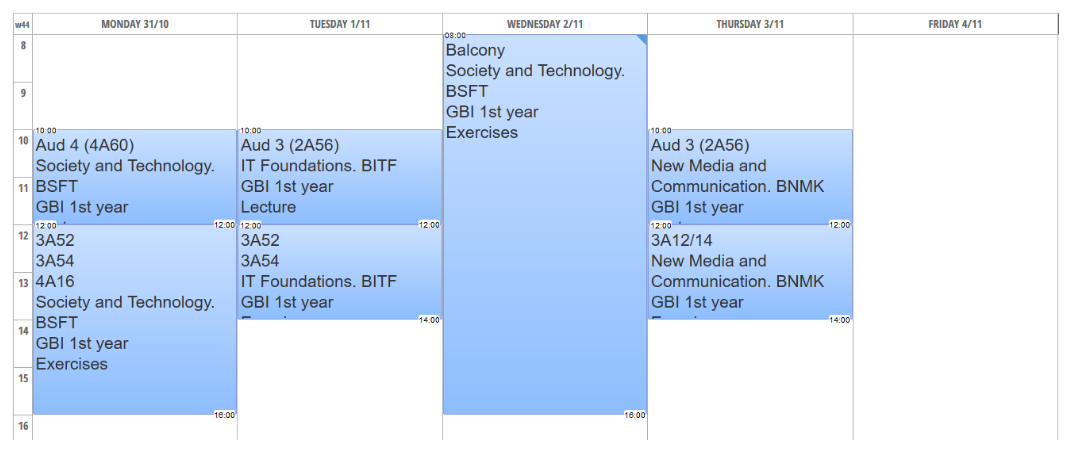
\includegraphics[width=\linewidth]{figures/schema-from-timeedit.png}
	\caption{Timeedit Schema for a 1st year GBI student}
	\label{fig:timeedit_schema}
\end{figure}

\newpar One of the most difficult parts of creating this batch view was handling the difference between WiFi Clients and Access Points, and how readings should be mapped to these. The design we chose was to use Map-reduce over the readings, and make the mapper read in all the meta data in the beginning of the job. Then when mapping the readings the meta data is looked up in two local list, one for WiFi clients and one for Access Points. We decided on this approach since the meta data file was of limited size and did not grow as fast as the readings data, of which there came one new file each day. But this approach is not the most effective and if we had for example used Hive, the process of combining meta data to readings would have happened in a parallized fashion.

\newpar We also spend some time figuring out how to use Avro serialization and how to integrate Avro with Map-Reduce. Avro uses a JSON like schema to define the binary format, the data is in. Making lists of lists was especially difficult which was the case for the readings, and furthermore we needed to define two Avro schemas for the different types of data, before and after it was cleaned and transformed into the different types.